\chapter{Evaluation}\label{chap:evaluation}
This chapter contains the evaluation of each edge platform based on the explained evaluations criteria from chapter \ref{chap:evaluation-criteria}. This chapter is structured in such a way that the platforms receive an evaluation/assessment for each point individually while maintaining the order of the evaluation criteria from chapter \ref{chap:evaluation-criteria}.

%%%%%%%%%%%%%%%%%%%%%%%%%%%%%%%%%%%%%%%%%%%%%%%%%%%%%%%%%%%%%%%%%%%%%%%%%%%%%%%%%%%%%%%%%%%%
\subsection*{Access to peripheral devices}
\subsubsection*{k3s}\label{subsubsec:evaluation-peripheral-devices-k3s}
The edge computing platform k3s allows running applications access to the host/node hardware by running them in privileged mode. Privileged mode is not recommended and not necessary for the most containers. Example use cases which requires the container to run in privileged mode is the access to hardware like attached peripheral devices (e.g. \gls{usb} dongle). Containers which are running in privileged mode can perform all the capabilities that it's host can. In basic terms, running privileged containers is like running an application as root in the host, which grants the container direct access to the kernel, hardware resources and mounted disks which may result into a security risk \cite{DockerRunReference} \cite{Cardoso2020}. 

\bigskip
An alternative is a Kubernetes device plugin. Kubernetes provides a device plugin framework that can be used to provide access to system hardware resources by advertising it to the Kubelet. Vendors can implement a device plugin that gets deployed either manually or as a DaemonSet which can then be used by running pods \cite{KubernetesDevicePlugins}.

\subsubsection*{AWS IoT Greengrass}
AWS IoT Greengrass has three different kinds of running applications. Each of the three possibilities allows access to peripheral devices like a \gls{usb} device. The simple one is the execution directly on the host without any isolation techniques. In this scenario, the user who executes the component needs this permission to access the requested hardware. The second option is executing the component as serverless function (AWS lambda). To get access to a device outside the lambda environment, the configuration during the component creation needs to be adjusted. Respectively by creating a lambda Greengrass component, the option of adding devices is given. This option can be used to add specific device paths like the one for \gls{usb} (e.g. \textit{/dev/bus/usb}) to the lambda environment. This option also allows setting the permission to read-only or to read-write. By deploying a serverless function with such a configuration, the Greengrass core device will handle all the necessary steps for giving the lambda access to the configured peripheral device. The last and third option is running the component as Docker container. To access peripheral devices like \gls{usb} from the inside of docker containers, the container requires to be run with the privileged flag, which sets the container in privileged mode. The k3s section \ref{subsubsec:evaluation-peripheral-devices-k3s}, before this section, already describes the problems by running containers in privileged mode.

\subsubsection*{ioFog}
ioFog runs its applications as docker containers, therefore like the k3s evaluation section of this evaluation criteria already points out the container needs to be run in privileged mode to be able to access peripheral devices from the inside of a container. The k3s section \ref{subsubsec:evaluation-peripheral-devices-k3s} also describes the problems by running containers in privileged mode.

\bigskip
To prevent direct host access from the running application inside a container, ioFog provides extra microservices which serve as a \gls{HAL}. This moves the privileged mode from the application container to the \gls{HAL} microservice and makes the device accessible over the \gls{HAL} microservice \cite{ioFogHALMicroservice}.
%%%%%%%%%%%%%%%%%%%%%%%%%%%%%%%%%%%%%%%%%%%%%%%%%%%%%%%%%%%%%%%%%%%%%%%%%%%%%%%%%%%%%%%%%%%%
\subsection*{Data Persistence}
\subsubsection*{k3s}
Persisting data can be done like in any other Kubernetes cluster. One way of storing data on a Kubernetes cluster is to use persistent volumes. These volumes provide a persistent storage, but no redundancy across the entire cluster if they are set up with the default storage class. Redundancy can be achieved by using a different storage class \cite{KubernetesDocsPersistentVolumes}. In the documentation of k3s, the storage class Longhorn\footnote{\url{https://longhorn.io/}} is recommended for redundancy. Longhorn is an open-source distributed block storage system for Kubernetes and is not included in k3s. Therefore, Longhorn must be installed manually by using the shell command from listing \ref{lst:eval-k3s-pv} \cite{k3sDocsPersistentVolumes}.

\begin{lstlisting}[caption={Installing Longhorn to k3s cluster \cite{k3sDocsPersistentVolumes}.},label={lst:eval-k3s-pv},captionpos=b]
kubectl apply -f https://raw.githubusercontent.com/longhorn/longhorn/ master/deploy/longhorn.yaml
\end{lstlisting}

\subsubsection*{AWS IoT Greengrass}
AWS Greengrass core devices are not meant to permanently store data on their disk. Greengrass core devices are meant to transform and react to incoming data. To store data, a viable way is to transfer the data to the AWS cloud and store it there. In principle, it is not impossible to store data to the core device's disk. To be more clear, it is possible to store data on the core device's disk by either mounting a local path into a container/lambada or by writing files to the disk if the component is executed directly on the host without any abstraction/isolation. This kind of storing data on the Greengrass core device does not contain any redundancy or security measures.

\subsubsection*{ioFog}
The edge computing platform ioFog is not really meant to permanently store data on the agent's disk. Like AWS IoT Greengrass local volumes can be mounted to microservices but local volumes are not replicated and therefore do not support redundancy features. A viable way would be to send data, which needs to be permanently stored, to a cloud. Another viable solution would be to maintain a NAS server in the local network, which can be used by the agents to store data. 

%%%%%%%%%%%%%%%%%%%%%%%%%%%%%%%%%%%%%%%%%%%%%%%%%%%%%%%%%%%%%%%%%%%%%%%%%%%%%%%%%%%%%%%%%%%%
\subsection*{Development Environment}
\subsubsection*{k3s}\label{subsubsec:eval-development-environmemt-k3s}
Developing services for k3s is like developing services for any Kubernetes cluster, or generally developing containerized applications. A local development environment can be set up by either deploying k3s in virtual machines like EC2 instances on \gls{AWS} or by using a development tool called k3d. The virtual machine option is the closest to the production environment. K3s can be installed on the virtual machines in the same way as on, e.g. on Raspberry Pi's. Even the ARM architecture can be represented, e.g. by using AWS Graviton\footnote{\url{https://aws.amazon.com/ec2/graviton/}} EC2 instances. The second option is by using the tool k3d, which is provided by the k3s vendor himself. K3d allows the developer to install a k3s cluster on a single machine. K3d only requires Docker to be installed on the development machine \cite{RancherDocsAdvancedOptions}. Depending on the size of the k3s cluster, it can consume a lot of resources on the host machine. Deploying a subset of the services may help to improve the performance of the development machine.
    
\subsubsection*{AWS IoT Greengrass}
Developing services, or components as AWS Greengrass calls them, can be done in three different ways. The Docker option is like in k3s  (\ref{subsubsec:eval-development-environmemt-k3s}). The option of simply executing a binary or script on the host itself is also painless. The last option, AWS lambda, can be tricky to test and develop. If the target device, the Greengrass core device, uses an ARM based CPU architecture, the development of a lambda may needs some tricks to work. If the developed lambda uses any native code e.g. through a third party library, the uploaded ZIP needs to contain the ARM native binaries and not the x86 binaries. Even the by \gls{AWS} provided command line tool \gls{SAM} is not able to target a specific CPU architecture. \gls{SAM} always targets x86 machines. As a workaround, the compiled native code needs to be replaced by ARM compiled code. Another pain during the development is the testing of components which use \gls{IPC} to communicate with other services. There is no mock or anything which can be used to test the component. One option would be to develop and run the component on a local Greengrass core device.

\bigskip
A local Greengrass core device can be set up by either using a virtual machine or by using a local Docker daemon. Nevertheless, the local core device needs to be registered in the \gls{AWS} console as Greengrass core device \cite{AWSGGCInDocker}. Components can then be added to the device by using the Greengrass core command line tool on the core device.

\subsubsection*{ioFog}
The edge computing platform ioFog allows the developer to set up a local development environment by deploying the control plane and agents to a locally running Docker daemon \cite{ioFogLocalDeployment}. A deployment to any virtual machine or similar is also possible. Microservices in ioFog are containerized applications. There is also an SDK which enables the microservice to use the internal message routing of the so called ioMessages. To test sending and receiving of ioMessages, parts of the ioFog SDK must be mocked, or the testing takes place inside a development environment. 

%%%%%%%%%%%%%%%%%%%%%%%%%%%%%%%%%%%%%%%%%%%%%%%%%%%%%%%%%%%%%%%%%%%%%%%%%%%%%%%%%%%%%%%%%%%%
\subsection*{Extensibility}
\subsubsection*{k3s} New nodes can be added with ease. The master node contains the so-called \textit{node-token} which allows new nodes to join the cluster by using this token. The \textit{node-token} can be obtained on the master and needs then be used upon starting the agent on the new node like shown in listing \ref{lst:k3s-join-node} \cite{k3s}. This method requires a pre-installed k3s executable on the new machine. Another way, which was also done for this evaluation, is to add an additional IP address to the \textit{hosts.ini} file to provision it with the tool Ansible.

\begin{lstlisting}[caption={Joining new node to k3s cluster.},label={lst:k3s-join-node},captionpos=b]
    sudo k3s agent --server https://<master>:6443 --token ${NODE_TOKEN}
\end{lstlisting}

\subsubsection*{AWS IoT Greengrass}
Adding new core devices to AWS IoT Greengrass can be easily done by running the Greengrass core installer on the respective new device. If the installer specifies an existing "\textit{Things Group}" the new core device will join this group and automatically runs the deployment for this group. Like in the implementation section (\ref{subsubsec:aws-ggc-devices}) of \gls{AWS} Greengrass mentioned, runtimes like Docker or Python won't get installed by the Greengrass core installer and must be therefore installed manually.

\subsubsection*{ioFog}
To add a new agent/node to the ioFog \gls{ECN} a new configuration file must be created. The configuration file can then be executed using the ioFog command line tool. The command line tool will then install all the necessary components on the node and then adds it to the \gls{ECN}. Unlike AWS Greengrass the ioFog command line tool also installs all necessary runtimes. One problem which can occur by adding new agents to the \gls{ECN} is the rising amount of YAML configuration files needed. For example, a fleet of 100 devices results into at least 100 YAML configuration files for just deploying the agent's default deamon and services. Adding one microservice to each of the agents will result in 100 additional configuration files. This mess with that many configuration files is a problem but will be addressed in future version (v3.0) of ioFog which is currently in alpha state \cite{ioFogTemplateEngine}.

%%%%%%%%%%%%%%%%%%%%%%%%%%%%%%%%%%%%%%%%%%%%%%%%%%%%%%%%%%%%%%%%%%%%%%%%%%%%%%%%%%%%%%%%%%%%
\subsection*{Offline capability}
\subsubsection*{k3s}
The edge computing platform k3s can be fully operated in offline mode. At any point, from setting up the nodes to running applications, no internet connection is required at all. The cluster only needs a functional network to communicate with each other. Even new applications whose container images have not yet been downloaded do not need internet access. Container images can be pulled from a network reachable container registry. Therefore k3s can be operated completly offline.

\subsubsection*{AWS IoT Greengrass}
With AWS Greengrass fully offline capability is not given. Each core device gets instructions from the AWS data centers, and therefore a working internet connection is necessary. Also downloading/pulling new components during the deployment phase requires the Greengrass core devices to have access to the internet. The only offline capability which AWS Greengrass Core devices provide is the option to keep messages in a local queue until transmission is possible. This is optimal for edge devices which face internet outages from time to time. To sum it up AWS IoT Greengrass is not meant to run in environments where no internet connection is the norm.

\subsubsection*{ioFog}
Like the k3s edge computing platform, ioFog is able to operate fully offline. Which means, microservices can communictae with each other without any internet connection. New applications and their corresponding container images can be pulled from a container registry inside the local network. The only difference between k3s and ioFog, in the offline context, is the optional tree like network at ioFog which allows a network structure where the agents only need a connection to the control plane and not to each other agent inside the system.

%%%%%%%%%%%%%%%%%%%%%%%%%%%%%%%%%%%%%%%%%%%%%%%%%%%%%%%%%%%%%%%%%%%%%%%%%%%%%%%%%%%%%%%%%%%%
\subsection*{Cloud connectivity}
\subsubsection*{k3s}
Any kind of integrated cloud connectivity is not provided by k3s. But there are no restrictions on deploying nodes in the cloud. Therefore, it is possible to build a k3s cluster with a conjugation of edge and cloud nodes. The simultaneous deployment of nodes at the edge and in the cloud eliminates the advantage of the offline capability but enables other possibilites.

\subsubsection*{AWS IoT Greengrass}
Like the example implementation already shows, AWS Greengrass core devices are controlled from \gls{AWS} data centers. This deep integration of \gls{AWS} allows Greengrass components, which are running locally on a Greengrass core device, to interact with any \gls{AWS} service. An advantage of this deep integration is that separate credentials like the AWS Credentials are not necessary for interacting with AWS services. The component on the core devices authenticates itself by doing  mutual TLS (mTLS) with the X.509 certificate of the core device. Which services the Greengrass component can access depends on the IAM role assigned to the core device. AWS SDKs like the boto3 Python SDK automatically use this mechanism to access AWS services \cite{AWSGGCInteractWithServices}. Therefore, a combination of edge computing and cloud computing can be achived.

\subsubsection*{ioFog}
The edge computing platform ioFog does not provide any integrated cloud connectivity. On the other side, the ioFog documentation recommends deploying the control plane into the cloud. A conjungtion of cloud and edge is also possible as well as deploying everything to the edge \cite{ioFogArchitecture}.
%%%%%%%%%%%%%%%%%%%%%%%%%%%%%%%%%%%%%%%%%%%%%%%%%%%%%%%%%%%%%%%%%%%%%%%%%%%%%%%%%%%%%%%%%%%%
\subsection*{Service Differentiation}
\subsubsection*{k3s} 
By adding resource limits to a pod, a kind of prioritization can be achieved. It is possible to define the CPU shares, which gives the container access to a greater or lesser proportion of the host machine’s CPU cycles. Listing \ref{lst:k3s-service-differentation} demonstrates the request of the CPU share value of 1024 \cite{DockerDocsResourceConstraints} \cite{KubernetesResourceConstraints}. Besides the CPU share prioritization, a prioritization for preemption and scheduling can be defined for each pod. This priority indicates the importance of a pod relative to other pods. If a pod cannot be scheduled, the scheduler tries to preempt (evict) lower priority pods to make scheduling of the pending pod possible \cite{KubernetesPriorityAndPreemption}.

\begin{lstlisting}[caption={Running pod with the CPU share value of 1024.},label={lst:k3s-service-differentation},captionpos=b]
---
apiVersion: v1
kind: Pod
metadata:
  name: app
spec:
  containers:
    - name: app
    image: <container_image>:<tag>
    resources:
      requests:
        cpu: 1
\end{lstlisting}
    
\subsubsection*{AWS IoT Greengrass}
There is no built-in feature for giving Greengrass components different priorities. Different component priorities can be achieved by using the runtime environment options. By running components directly on the core device without abstraction/isolation, the scheduling priority can be modified by increasing or decreasing the niceness value of the corresponding process. Nicenesses range from -20 (most favorable scheduling) to 19 (least favorable) \cite{nice}. Docker containers can also be started with a type of priority. By adding the flag "\textit{--cpu-shares <number>}", like in listing \ref{lst:aws-service-differentation}, to the run command, Docker gives the container access to a greater or lesser proportion of the host machine’s CPU cycles \cite{DockerDocsResourceConstraints}.

\begin{lstlisting}[caption={Running Docker container with less shares than the default \cite{DockerDocsResourceConstraints}.},label={lst:aws-service-differentation},captionpos=b]
docker run -d --cpu-shares 512 <container_image>:<tag>
\end{lstlisting}
    
\subsubsection*{ioFog}
The possibility to specify CPU shares, like in k3s and AWS IoT Greengrass, is not possible for ioFog microservices. In general, there is no option to give a microservice any kind of prioritization relative to other microservices. The only prioritization which can be made is the priotiry attribute on each ioMessages. This assigned priority functions as a simple quality of service (QoS) indicator \cite{ioFogAgentReference}.
%%%%%%%%%%%%%%%%%%%%%%%%%%%%%%%%%%%%%%%%%%%%%%%%%%%%%%%%%%%%%%%%%%%%%%%%%%%%%%%%%%%%%%%%%%%%
\subsection*{Reliability}
\subsubsection*{k3s}
By unplugging one node, not the master/control plane, from the example setup, this node will be marked as \textit{"NotReady"} in the status field. The listing \ref{lst:k3s-unplug-node} shows the command line output while one worker node is unplugged.

\begin{lstlisting}[caption={Status of node 1 while unplugged.},label={lst:k3s-unplug-node},captionpos=b]
> kubectl get nodes
NAME     STATUS     ROLES                  AGE   VERSION
master   Ready      control-plane,master   5d    v1.21.1+k3s1
node1    NotReady   <none>                 5d    v1.21.1+k3s1
node2    Ready      <none>                 5d    v1.21.1+k3s1
\end{lstlisting}

Pods form the unplugged node (not ready) get moved to running nodes by recreating them. This can be seen by unplugging one node and then periodically fetching the pod states e.g. with \textit{kubectl}. Nodes which are specific to one node due to pod selection won't get recreated if there is no other pod which matches the given node selector. One must keep in mind that volumes are stored to the node disk itself, with the default storage class. To be able to move pods, which require persistent storage, a storage driver with redundancy support must be used.

\bigskip
The reliability of individual pods can be managed too. By adding liveness, readiness and startup probes for pods the cluster can detect failing pods.
In addition to the probes, a restart policy can be attached to a pod which tells the cluster on which failure events it should restart the pod. It defaults to restart the pod on each failure. This can be configured for each pod individually. Restarts happen with an exponential back-off delay (10s, 20s, 40s, …), that is capped at five minutes \cite{KubernetesPodLifecycle}.

\subsubsection*{AWS IoT Greengrass}
Failing Greengrass components or unavailable Greengrass core devices get marked as \textit{"UNHEALTHY"} in the AWS IoT Core Console. By loosing a Greengrass core device, the impact to the entire system depends on the system architecture. For example, a system for a postal service with one Greengrass core device on each delivery truck will result into entire lose of control for this truck. This is because no backup is available, so the control to this truck is lost until the core device reestablishes connection. A different example is the one which was built in the implementation section. Loosing one of the nodes, which was tested by unplugging one node, causes the sensors and actors to switch to healthy nodes. This switch can only be done if a healthy core device is in reach of the sensors which lost their initial core device.

\subsubsection*{ioFog}
The very granular control of microservice deployment to selected agents does not allow the move of microservices to healthy agents. To be more general, ioFog's agents do not work in cluster mode and therefore no auto recovery like in Kubernetes can be done. It's only possible to inform the system administrators about the failing/unavailable agent. Failing microservices are detectable over the ioFog API based on the status field. Sensor can switch the agen but the switching must be implemented by the developers.
%%%%%%%%%%%%%%%%%%%%%%%%%%%%%%%%%%%%%%%%%%%%%%%%%%%%%%%%%%%%%%%%%%%%%%%%%%%%%%%%%%%%%%%%%%%%
\subsection*{Security}
\subsubsection*{k3s}
Encryption is not used by default. For example, network encryption depends on the used \gls{CNI}. The default \gls{CNI} is VXLAN which is not encrypted. The following table \ref{tap:k3s-flannel-options} gives a brief overview of all available options to choose from for the \gls{CNI} including encrypted network options. Custom \gls{CNI}'s can be used too, but must be installed manually \cite{k3sNetworkOptions}. Encryption outside the cluster like the connection between the sensor to the MQTT broker, from the example implementation, must be enabled/configured by the developer themselves.

\begin{table}[H]
\centering
\begin{tabular}{|p{0.35\linewidth}|p{0.58\linewidth}|} \hline
    \textbf{CLI Flag and Value} & \textbf{Description} \\ \hline
    ---flannel-backend=vxlan     & (Default) Uses the VXLAN backend. \\ \hline
    ---flannel-backend=ipsec     & Uses the IPSEC backend which encrypts network traffic. \\ \hline
    ---flannel-backend=host-gw   & Uses the host-gw backend. \\ \hline
    ---flannel-backend=wireguard & Uses the WireGuard backend which encrypts network traffic. May require additional kernel modules and configuration. \\ \hline
\end{tabular}
\caption{Flannel backend CLI options \cite{k3sNetworkOptions}.}\label{tap:k3s-flannel-options}
\end{table}

\subsubsection*{AWS IoT Greengrass}
In AWS IoT Greengrass every communication, except the inter process communication between components on the core device, is encrypted. Each AWS Thing like a Greengrass core device have their own certificates and keys which get used on every communication step. The built-in MQTT broker only allows secure connections by default. In addition, the MQTT broker also requires the MQTT client to use mutual TLS (mTLS) protocol to authenticate them. Mutual TLS is also used by the Greengrass core devices for every communication from and to the cloud. The certificate from each device is attached to an AWS IAM role, which defines the operations allowed for AWS IoT devices \cite{AWSGGCEncryptionInTransit} \cite{AWSGGCDeviceAuth}.

\subsubsection*{ioFog}
The ioFog documentation does not mention any specific details about used security mechanism. By digging into the code of the agent\footnote{\url{https://github.com/eclipse-iofog/Agent/tree/v2.0.7}} and controller\footnote{\url{https://github.com/eclipse-iofog/Controller/tree/v2.0.1}}, the following security mechanism were found. The controller and agent communicate over HTTPS by using their self-signed certificates. The agent always pins the certificate on each request, which means it checks if the controller is really the one that it claims to be. Additionally, security guidelines are enforced and controlled by every node. Which guidelines are enforced and checked exactly are not further mentioned \cite{Marshall2019}. External communication is not secured by default and must be therefore done by the developer by e.g. using an MQTT broker in TLS mode.

%%%%%%%%%%%%%%%%%%%%%%%%%%%%%%%%%%%%%%%%%%%%%%%%%%%%%%%%%%%%%%%%%%%%%%%%%%%%%%%%%%%%%%%%%%%%
\subsection*{Real-time capability}
\subsubsection*{k3s}
The edge computing platform has no built-in messaging solution therefore normal HTTP request were made to meassure the overall latency. Two pods, ping and pong, were deployed on two different nodes of the k3s cluster to meassure the latency between them. Figure \ref{fig:k3s-latency} shows the meassureing results in milliseconds. Compared to its competitotrs the overall latency is highest of all of them. Therefore, a kind of real-time messaging is not possible/recommended with this latency.

\begin{figure}[H]
    \centering
    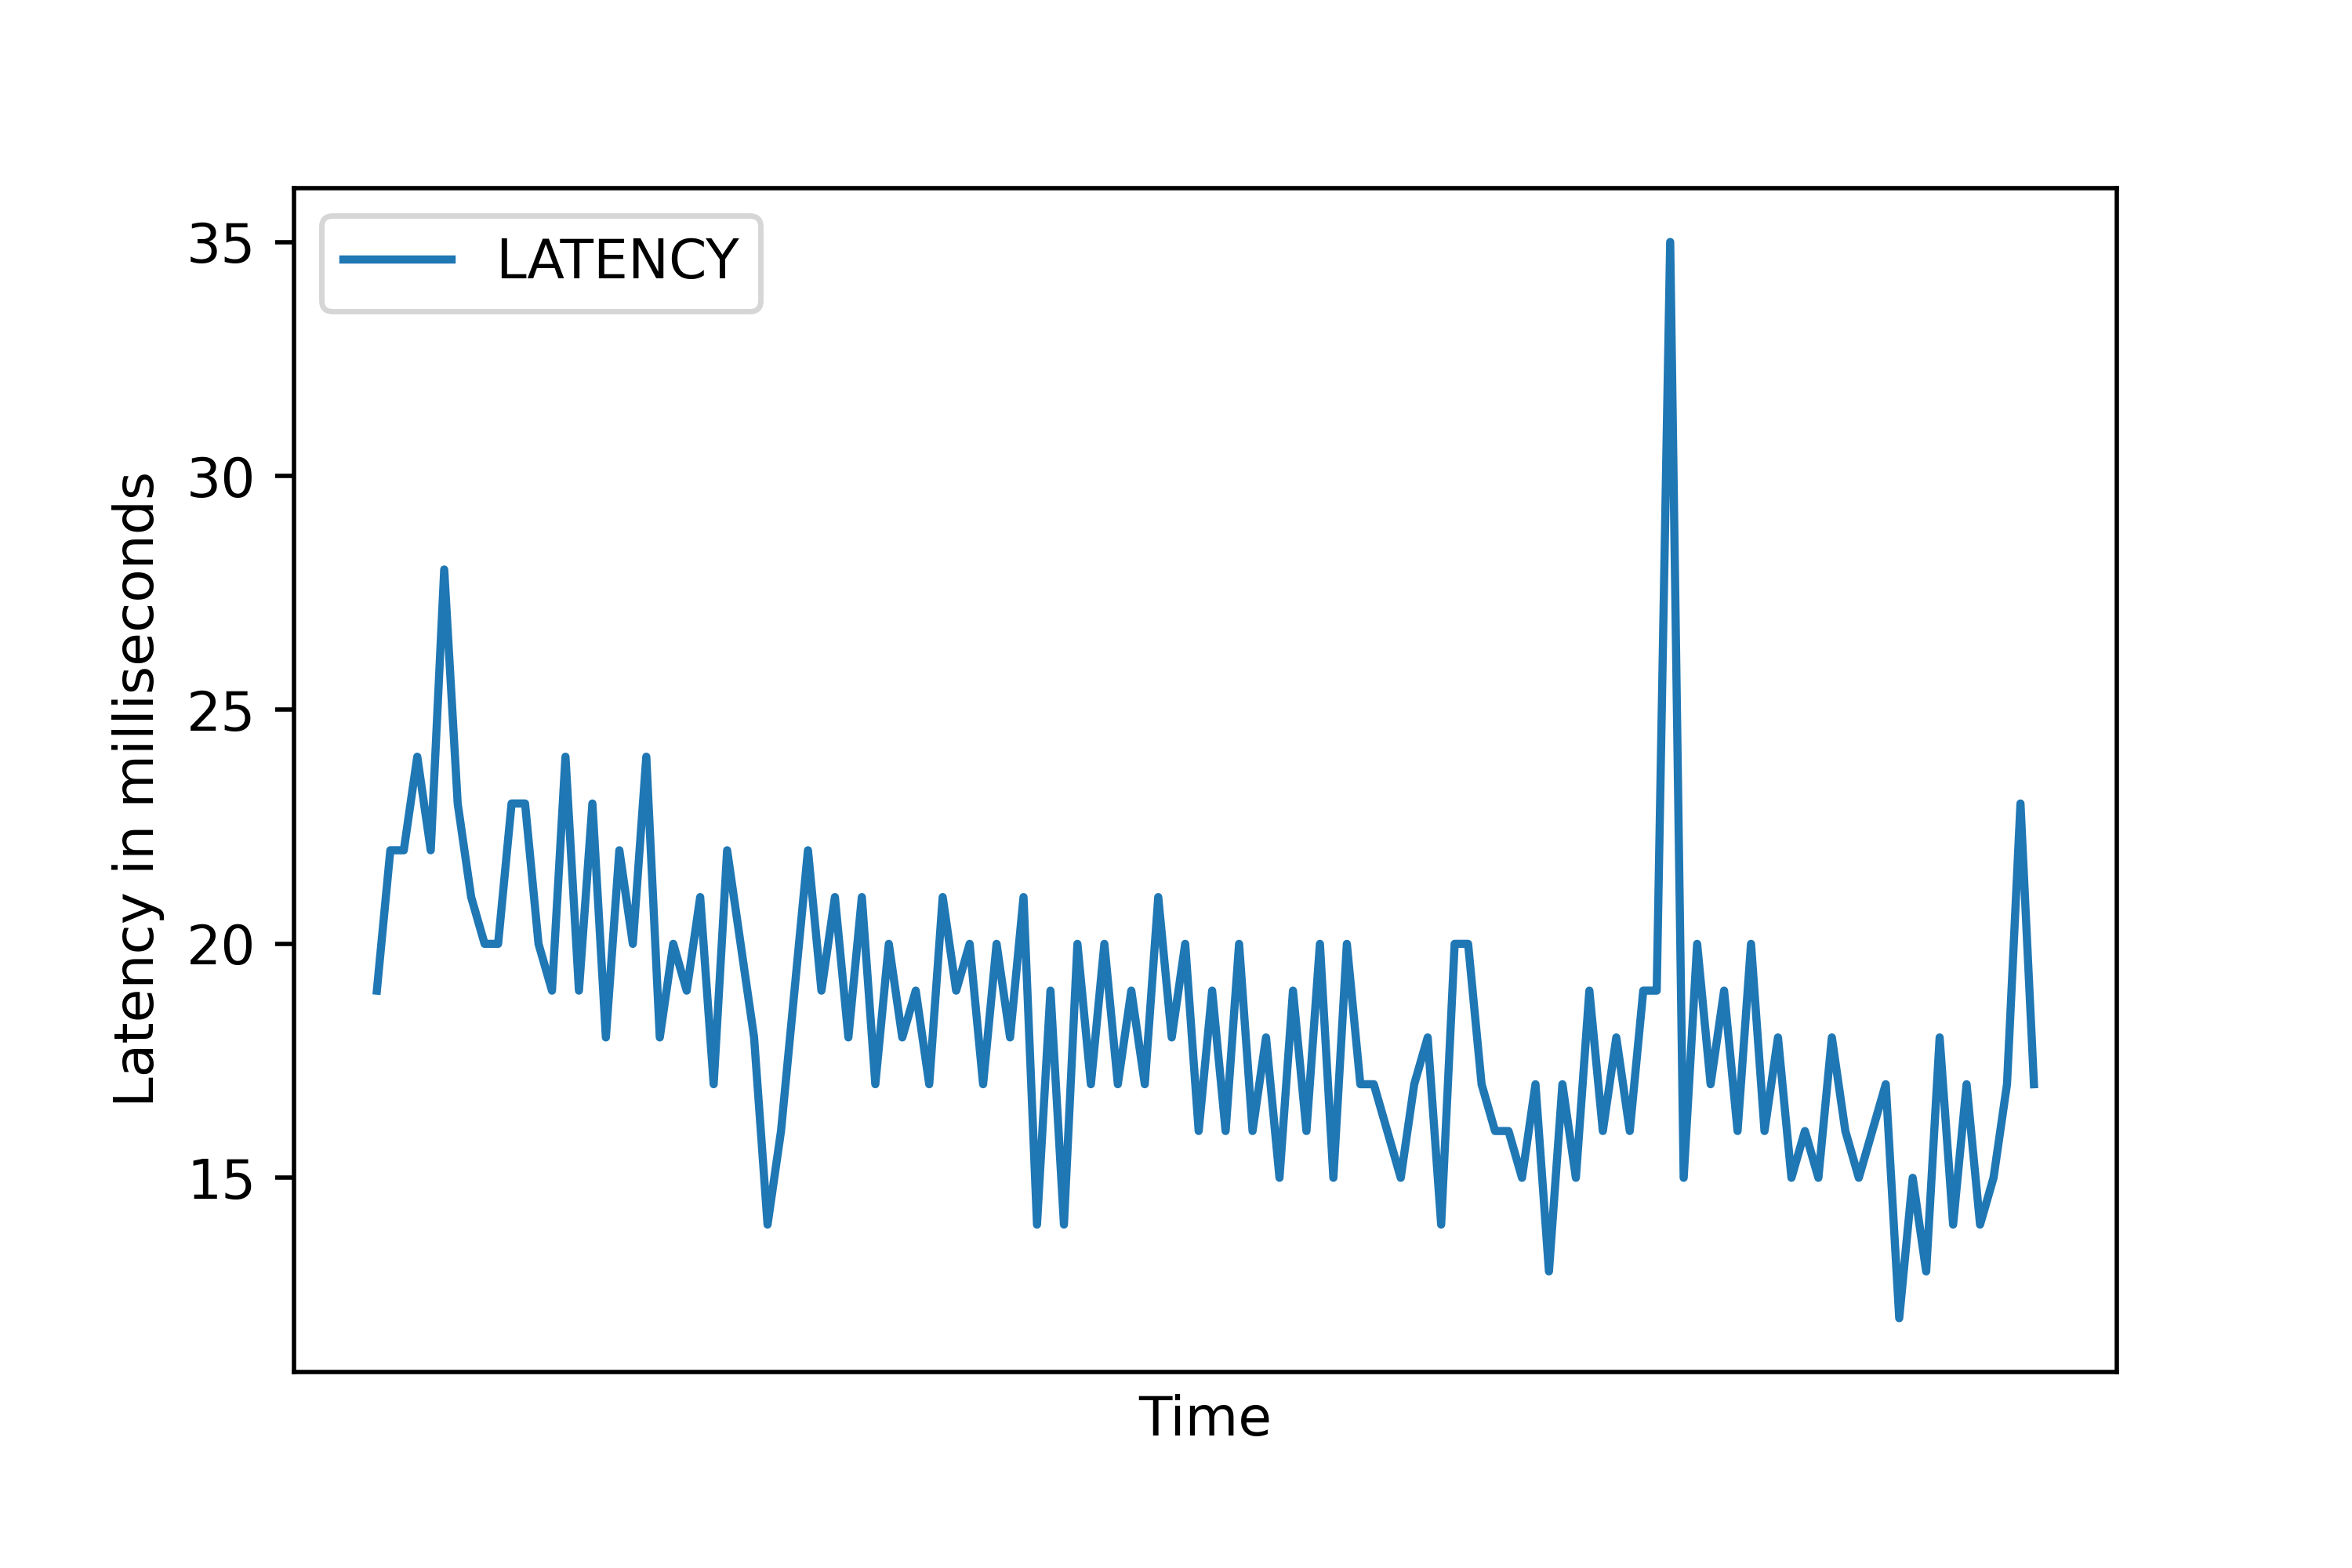
\includegraphics[width=0.8\textwidth]{assets/k3s/latency/plots/latency.png}
    \caption{HTTP latency between two pods on two nodes.}\label{fig:k3s-latency}
\end{figure}

\subsubsection*{AWS IoT Greengrass}
By using the \gls{IPC} provided on each Greengrass core device the latency is very low with some exceptions. Figure \ref{fig:aws-iomessage-latency} shows a message latency plot of two Greengrass components communicating over the built-in \gls{IPC} interface. Before the measuring was done, the core device got a fresh installation of the Greengrass core device components. The response time of around 4 milliseconds is good enough to deliver messages from high priority fast enough.

\begin{figure}[H]
    \centering
    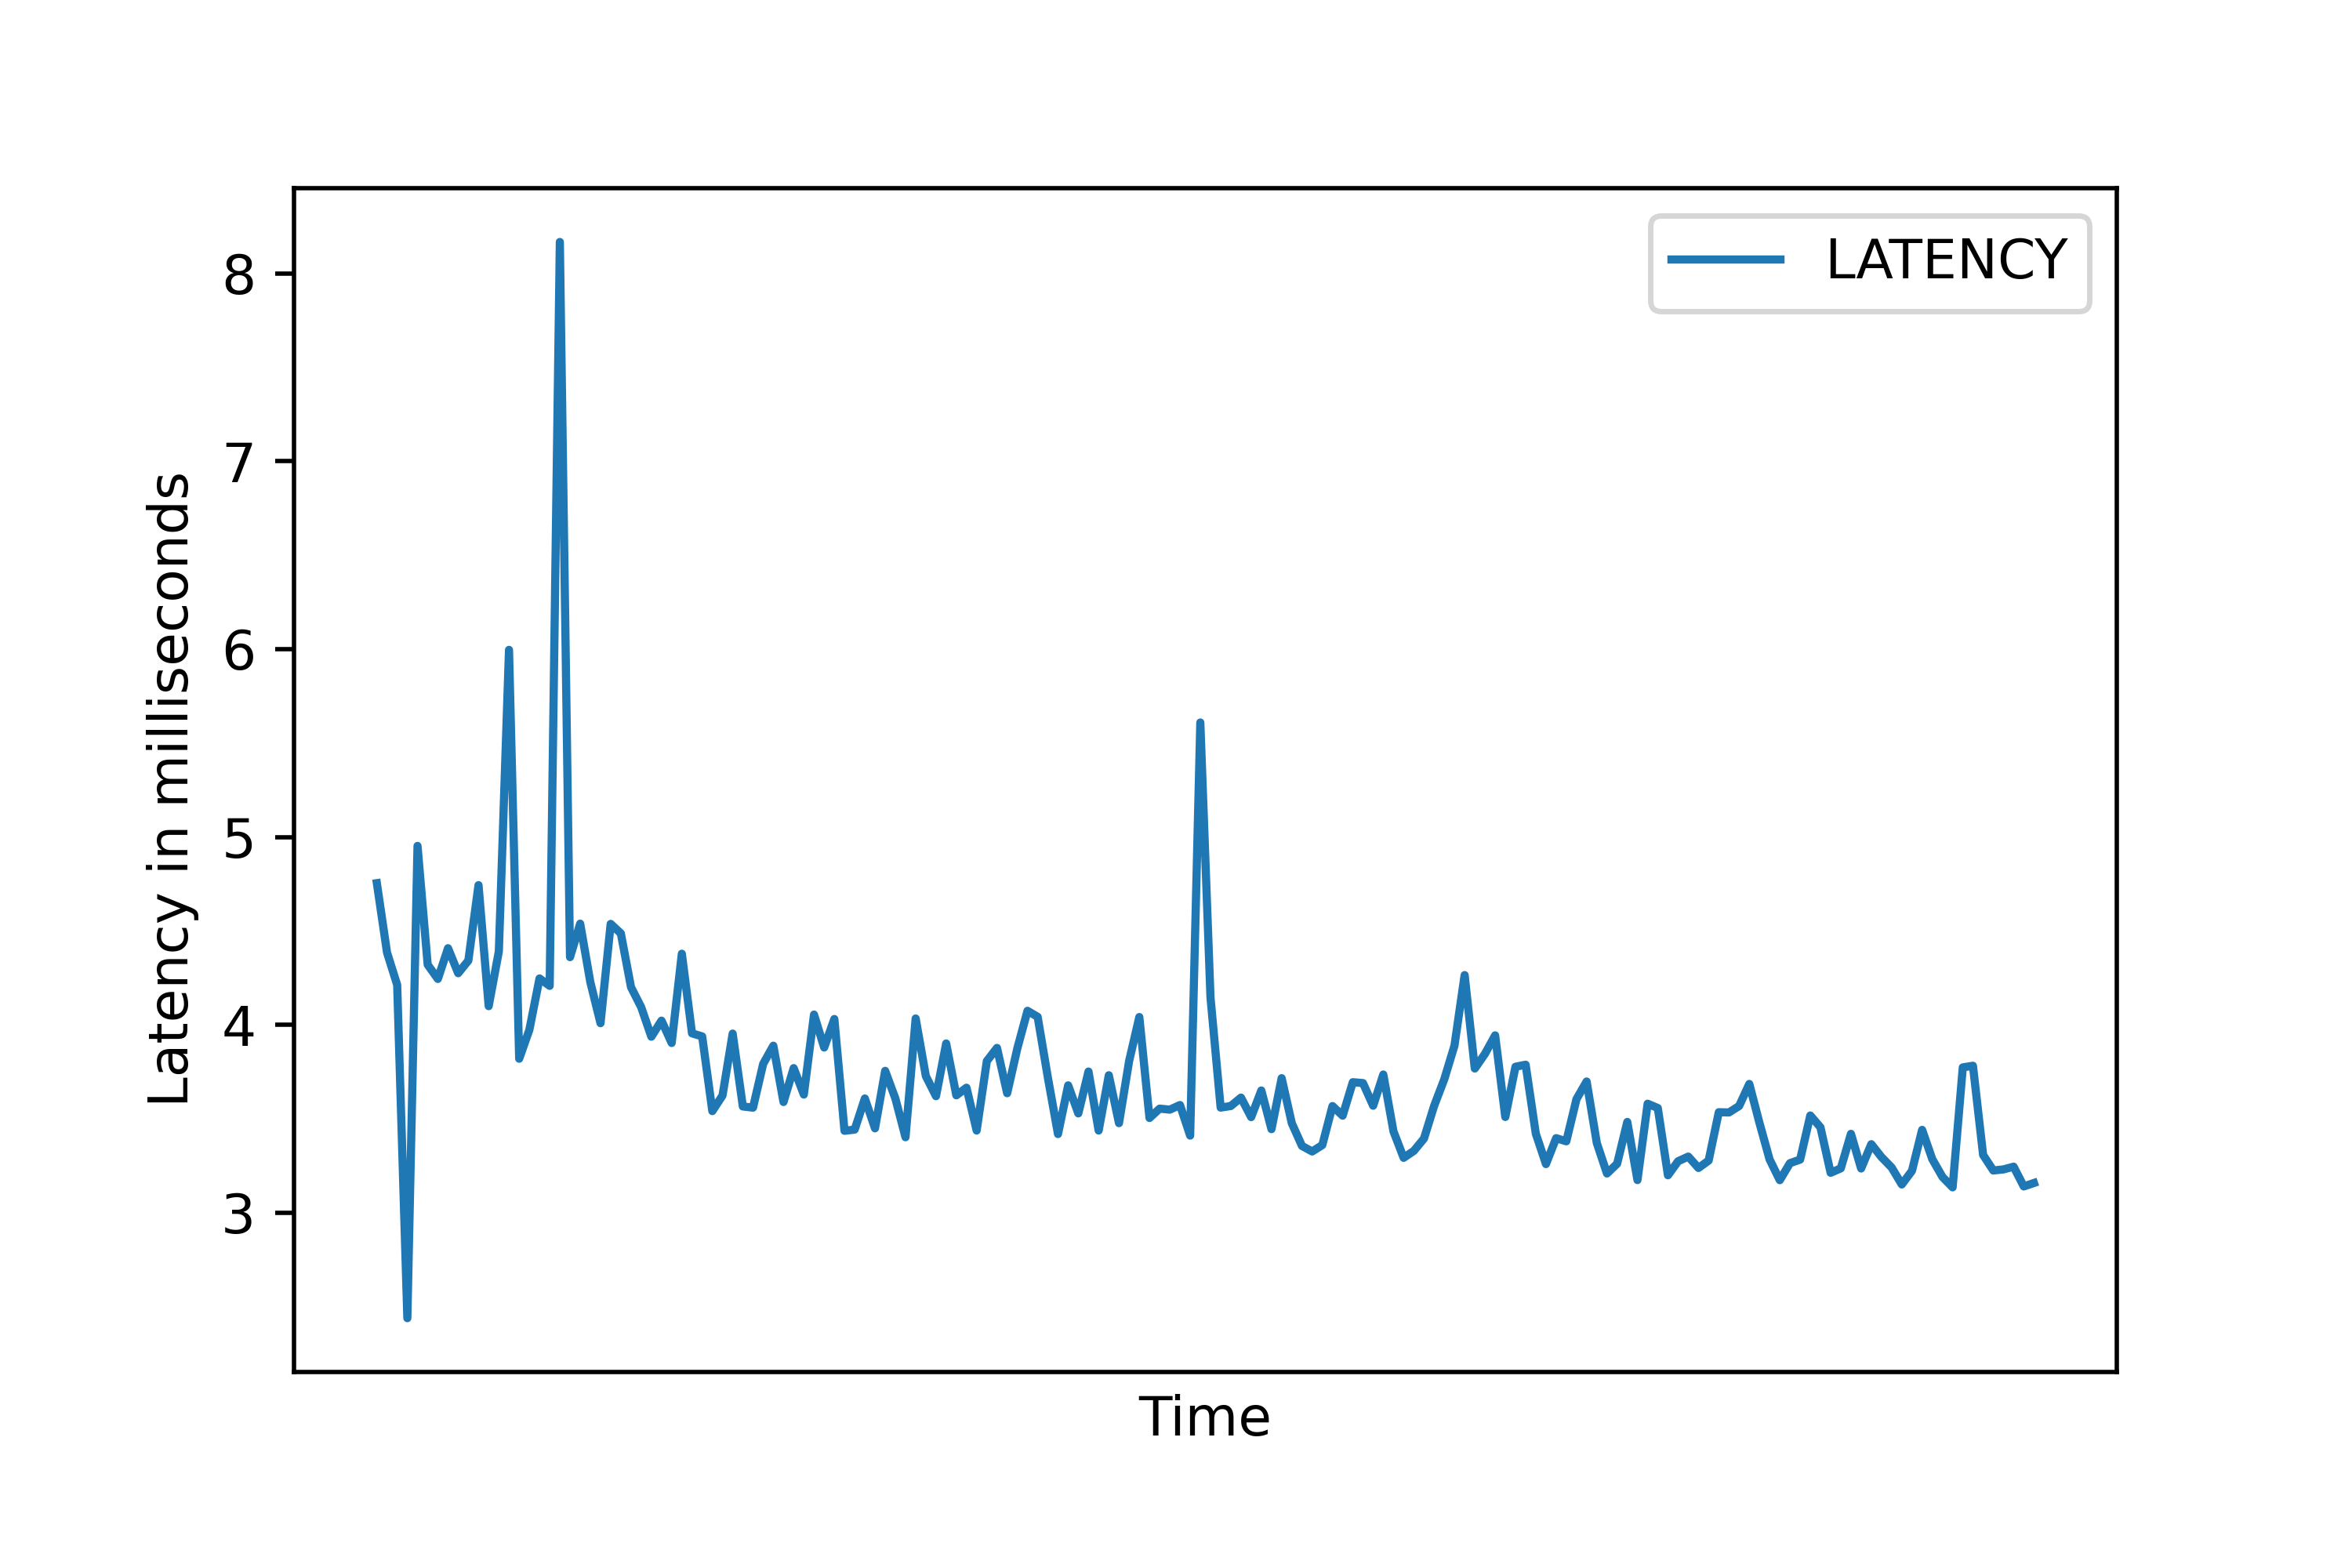
\includegraphics[width=0.8\textwidth]{assets/aws-greengrass/latency/plots/latency.png}
    \caption{IPC latency between two components on the same core device.}\label{fig:aws-iomessage-latency}
\end{figure}

\subsubsection*{ioFog}
By using the built-in messaging system of ioFog the latency can vary a lot like figure \ref{fig:ioFog-iomessage-latency} indicates. The recorded data points is the messaging time between two microservices on the same agent. Before the recording was done, the agent got a fresh installation of the ioFog agent services and daemons. The high spikes on an agent with just two microservices is not really promising on the real-time point of view. Therefore, a kind of real-time messaging is not possible/recommended with the native messaging system. Other options like communication inside the docker created network would make a better choice for a real time scenario.

\begin{figure}[H]
    \centering
    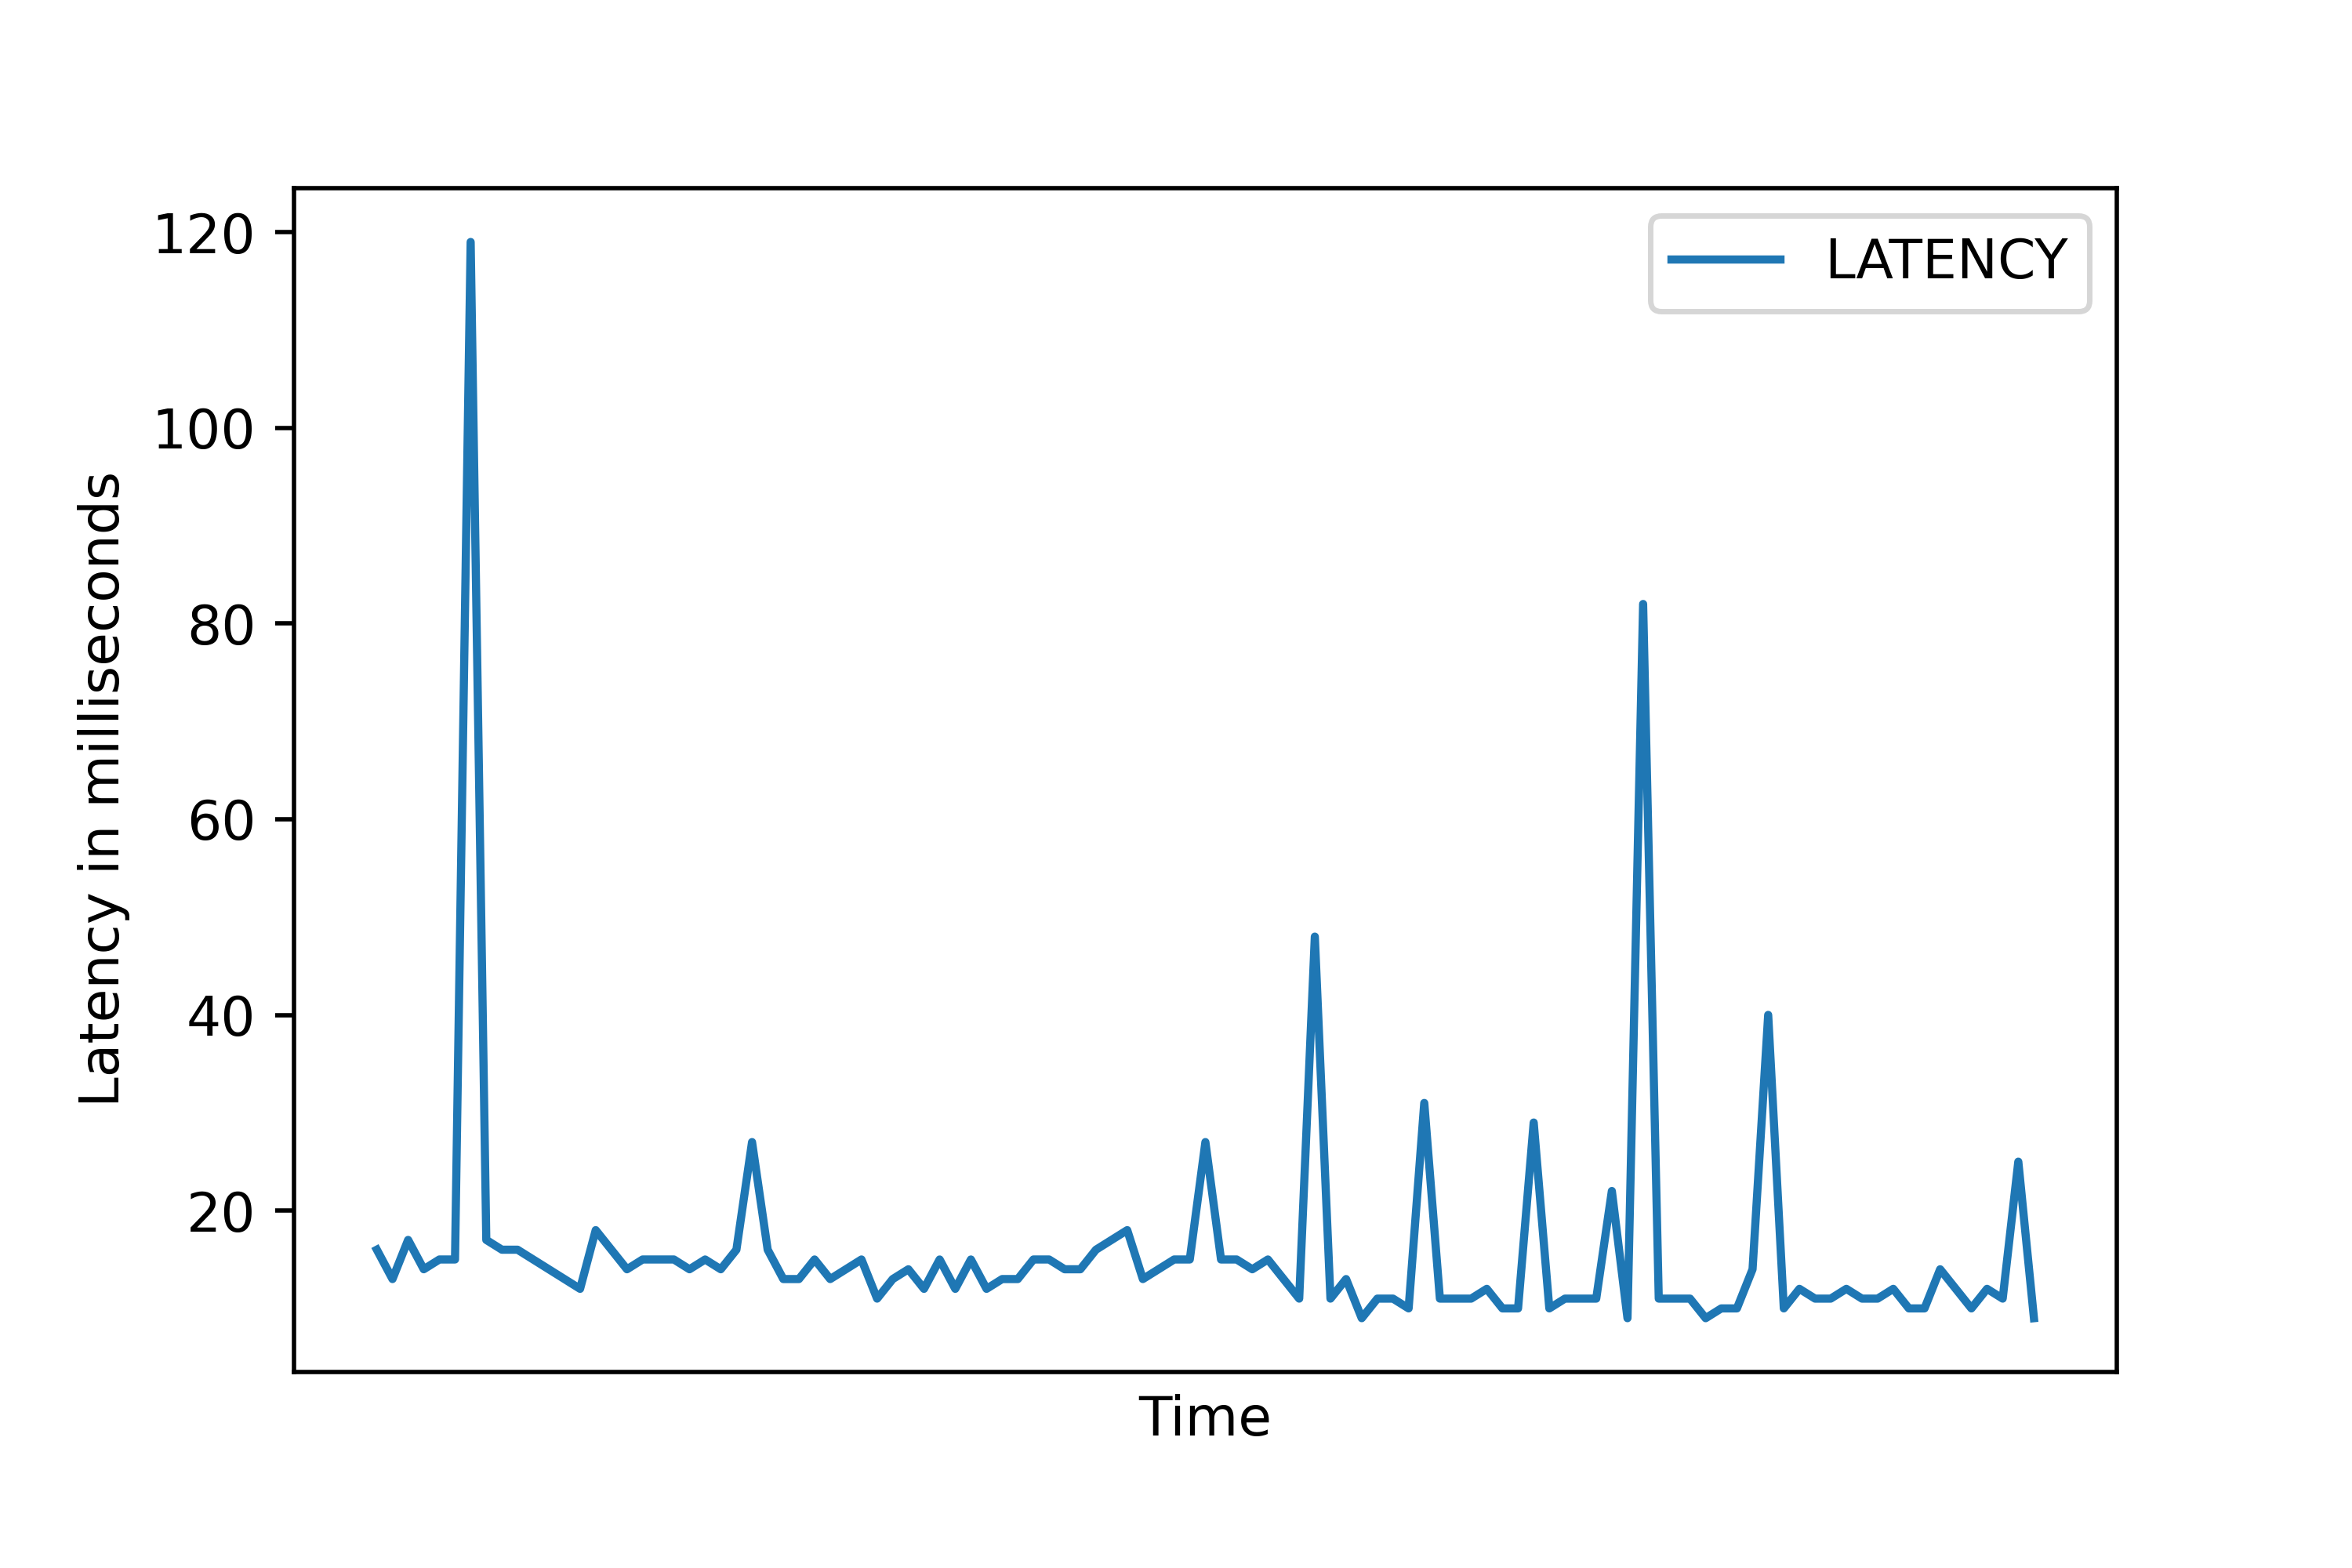
\includegraphics[width=0.8\textwidth]{assets/iofog/latency/plots/latency.png}
    \caption{ioMessage latency between two microservices on the same agent.}\label{fig:ioFog-iomessage-latency}
\end{figure}

%%%%%%%%%%%%%%%%%%%%%%%%%%%%%%%%%%%%%%%%%%%%%%%%%%%%%%%%%%%%%%%%%%%%%%%%%%%%%%%%%%%%%%%%%%%%
\subsection*{Performance}
Performance was measured by doing a fresh installation for each edge computing platform. No additional services were installed or added after the fresh installation. Performance is hard or even impossible to measure if it should be representative for each hardware. Therefore, an idling system was measured to show how much of the available resources each edge computing platform utilizes. The measuring was done with the Linux command line tool \textit{top}. The \textit{top} tool displays information about a selection of the active processes \cite{topUserManual}. The command from listing \ref{lst:performance-cli} was executed on each node for 15 minutes. The output file of the command from listing \ref{lst:performance-cli} was then transformed to draw the following plots.

\begin{lstlisting}[caption={Command to dump CPU and memory utilization.},label={lst:performance-cli},captionpos=b]
while true; do (echo "--- $(date)" && top -b -n 1 | head -n 5) >> ps.log; sleep 5; done
\end{lstlisting}

\subsubsection*{k3s}
The master node uses overall more memory and CPU time than the two worker nodes, as shown in figure \ref{fig:performance-k3s}. This is an expected behavior due to the fact that the master nodes contains several services to manage the cluster. The worker nodes utilize around the same amount of CPU and memory as expected. The usage of under 10\% of memory and CPU time, at the worker nodes, leaves plenty of resource for other services.

\begin{figure}[H]
    \centering
    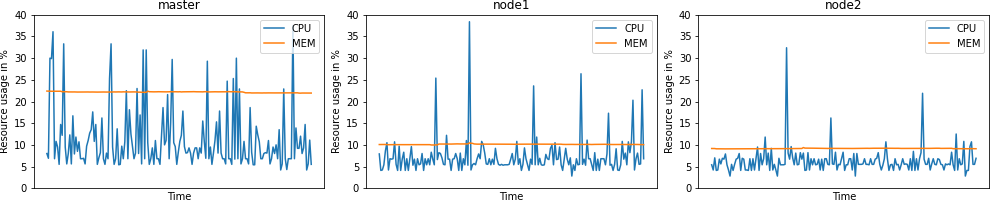
\includegraphics[width=\textwidth]{assets/k3s/logs/plots/results.png}
    \caption{CPU \& memory usage for the nodes master, node-1, node-2.}\label{fig:performance-k3s}
\end{figure}
    
\subsubsection*{AWS IoT Greengrass}
Each AWS Greengrass core devices contains the same set of services after a fresh installation, therefore the CPU and memory usage should be around the same amount. The plots in figure \ref{fig:performance-aws} confirm this assumption of nearly the same CPU and memory usage.

\begin{figure}[H]
    \centering
    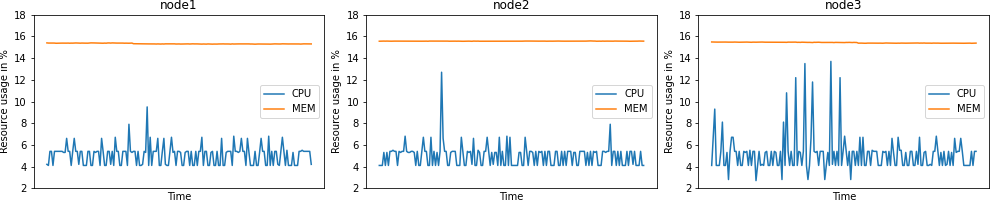
\includegraphics[width=\textwidth]{assets/aws-greengrass/logs/plots/results.png}
    \caption{CPU \& memory usage for the nodes node-1, node-2, node-3.}\label{fig:performance-aws}
\end{figure}

\subsubsection*{ioFog}
The CPU and memory usage across controller and agents seems to be around the same, as shown in the plots of figure \ref{fig:performance-ioFog}. The memory usage of around 20\% is high a may result into problems for memory intensive tasks compared to e.g. k3s.

\begin{figure}[H]
    \centering
    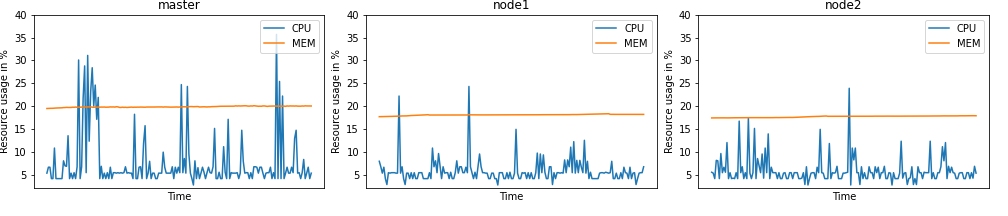
\includegraphics[width=\textwidth]{assets/iofog/logs/plots/results.png}
    \caption{CPU \& memory usage for the nodes master, node-1, node-2.}\label{fig:performance-ioFog}
\end{figure}

\subsubsection*{Summary}
The edge computing platform k3s seems to be the best in the category of the most balanced use of CPU and memory. The best in CPU is AWS IoT Greengrass closely followed by k3s. The most memory efficient platform is k3s. The ioFog edge computing platform seems to be the worst of all three, with its high memory usage and many high CPU usage spikes.

%%%%%%%%%%%%%%%%%%%%%%%%%%%%%%%%%%%%%%%%%%%%%%%%%%%%%%%%%%%%%%%%%%%%%%%%%%%%%%%%%%%%%%%%%%%%
\subsection*{Distributing workload}
\subsubsection*{k3s}
In short terms, its Kubernetes. The long explanation is the nature of Kubernetes and its workload distribution to all cluster nodes. Deploying an application into a Kubernetes cluster allows horizontal scaling. The horizontal scaling can be automated based on the load. This autoscaling feature of Kubernetes allows the system to dynamically react to increasing/decreasing demand of applications. By scaling up an application, creating replicas, the distribution to nodes is made by the kubelet. Mostly applications are normally not specifically targeted to one node, the kubelet then evenly distributes the applications to the available nodes in the cluster \cite{TheKubernetesAuthors}. 

\bigskip
One example of distributing workload at k3s is the MQTT broker cluster from the example implementation. The MQTT broker were deployed across all nodes to remain functional in the event of a node failure and also to get more computing resources if necessary. The workload was then distributed by adding a load balancer in front of the MQTT broker cluster. This load balancer evenly distributed all incoming connections to the available MQTT brokers.

\subsubsection*{AWS IoT Greengrass}
A distribution of workload is not the intention of AWS IoT Greengrass. Of course the distribution of workload can be implemented by the developer on their own, but this requires extra work to be done and isn't the default mode to compute things with AWS IoT Greengrass.

\subsubsection*{ioFog}
A distribution of workload is not the intention of ioFog. Doesn't mean it cannot be done. For example, having one agent which collects the sensor data in the area and distributes it to two nearby agents for the computational work. But this must be implemented by the developer and is not the default way.
%%%%%%%%%%%%%%%%%%%%%%%%%%%%%%%%%%%%%%%%%%%%%%%%%%%%%%%%%%%%%%%%%%%%%%%%%%%%%%%%%%%%%%%%%%%%
\subsection*{Energy Consumption}
For evaluating the overall energy consumption each system was measured for exactly one hour. One data point was recorded each second. Each platform was set up with three fresh installed nodes connected to the \gls{PoE} switch. The measuring was done on the \gls{PoE} switch power supply. Each system was idling and did not contain any custom applications or services, which do not come out of the box installed. Figure \ref{fig:energy-consumption-plot} presents the result from the experiment.

\begin{figure}[H]
    \centering
    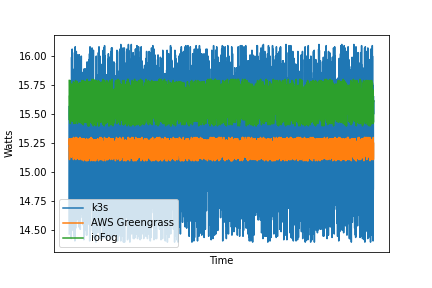
\includegraphics[width=\textwidth]{assets/evaluation/plots/energy-consumption.png}
    \caption{Energy consumption plot for all edge computing platforms.}\label{fig:energy-consumption-plot}
\end{figure}

\subsubsection*{k3s}
The energy consumption of k3s is varying a lot. Most of the energy is consumed by the node containing the control plane, as can be seen from the CPU and memory graphs in the first plot of the figure \ref{fig:performance-k3s} (the performance and energy consumption experiments were independent from each other).

\subsubsection*{AWS IoT Greengrass}
The AWS IoT Greengrass edge computing platform has the most consistent energy consumption of all platforms.

\subsubsection*{ioFog}
The power consumption of ioFog is very high compared to the rest considering that there are only two worker nodes available as the third is the designated to be the controller node.
%%%%%%%%%%%%%%%%%%%%%%%%%%%%%%%%%%%%%%%%%%%%%%%%%%%%%%%%%%%%%%%%%%%%%%%%%%%%%%%%%%%%%%%%%%%%
\subsection*{Cost}
Calculating the costs is more difficult than in the public cloud because hardware must be acquired, additional staff must be hired and more. The hardware cost also depends on the use case. For example, an edge computing use case which does a lot of machine learning task requires TPUs or GPUs which increases the cost where, on the other hand, sensor data processing requires less computing power which decreases the cost of hardware. And of course the size of the device fleet also plays an important role in the cost calculation.

\subsubsection*{k3s}
The costs are composed of the hardware and the additional staff members. Extra costs can be added if one of the node, e.g. the control plane, is deployed in a virtual machine at a public cloud like \gls{AWS}. But the entire system can be run locally without any cloud provider.
    
\subsubsection*{AWS IoT Greengrass}
Besides the hardware costs and the additional staff members, \gls{AWS} charges \$0.18\footnote{Price is taken from the region Europe(Frankfurt)} per month and Greengrass core device (price is varying depending on the region). Additionally, \gls{AWS} charges for AWS IoT Core connections e.g. transferring MQTT messages from and to the cloud, AWS \gls{S3} for storing application files, AWS \gls{ECR} for storing container images, and every other AWS services which is used by the core devices or components \cite{AWSGGCPricing}.

\subsubsection*{ioFog}
Like k3s the costs are composed of the hardware and the additional staff members. Agents or the control plane of ioFog can also be deployed to the cloud and will then generate additional cloud costs. But this is not necessary.
%%%%%%%%%%%%%%%%%%%%%%%%%%%%%%%%%%%%%%%%%%%%%%%%%%%%%%%%%%%%%%%%%%%%%%%%%%%%%%%%%%%%%%%%%%%%
